\chapter{Kinematics}\label{cha:kinematic}

In \chapref{cha:overview}, an overview of the system available on Aalborg university was introduced. In this chapter we derive the kinematics. This is done to describe each joint and end effector positions for e.g the Geomagic Touch or the hand of the da Vinci robot. 

In the following the \gls{DH} notation is going to be used\cite{spong2008robot}. This eases calculation of the different positions and gives a simple , unambiguous description of the kinematics using the least amount of parameters. The \gls{DH} notation only uses four parameters to describe the transformation between the different frames. Each joint is given its own coordinate frame do describe the link between the different joints and are denoted as $O_i$ from 0 to $n$. To utilize the \gls{DH} notation some rules got to be fulfilled and are as followed\cite{spong2008robot}:

\begin{itemize}
\item DH(1): The axis $x_n$ is perpendicular to axis $z_{n-1}$
\item DH(2): The axis $x_n$ intersects the axis $z_{n-1}$
\end{itemize}

furthermore the joints rotates around the z axis where the right hand rule is used.

The \gls{DH} convention is described through the transformation matrix shown in \eqref{equ:DH_trans_matrix}\cite{spong2008robot}. This matrix is calculated for each joint and gives the transformation and rotation. Note that $\sin()$ is denoted as $s$ and $\cos()$ is denoted as $c$.

\begin{equation}
\begin{split}
A_i  & = Rot_{z,\theta_{i}}Trans_{z,d_{i}}Trans_{x,a_{i}}Rot_{x,\alpha_{i}} \\
     & = \begin{bmatrix}c_{\theta_{i}} & -s_{\theta_{i}} & 0 & 0 \\ s_{\theta_{i}} & c_{\theta_{i}} & 0 & 0\\  0 &0 & 1 &0 \\ 0 &0&0& 1\end{bmatrix} 
      \begin{bmatrix}1 &0& 0& 0\\ 0& 1& 0& 0\\ 0& 0& 1& d_{i}\\ 0& 0& 0& 1\end{bmatrix} 
      \begin{bmatrix} 1 & 0 &0& a_{i}\\ 0& 1& 0 &0\\ 0 &0 &1& 0\\ 0 &0& 0 &1\end{bmatrix}
      \begin{bmatrix}1& 0& 0& 0\\0& c_{\alpha_{i}}& -s_{\alpha_{i}} & 0\\ 0 & s_{\alpha_{i}} & c_{\alpha_{i}} & 0\\ 0& 0 &0& 1 \end{bmatrix}\\
     & = \begin{bmatrix}c_{\theta_i}& -s_{\theta_i}c_{\alpha_i}& s_{\theta_i}s_{\alpha_i}& a_{i}c_{\theta_i}\\ s_{\theta_i}& c_{\theta_i}c_{\alpha_i} & -c_{\theta_i}s_{\alpha_i}& a_{i}s_{\theta_i}\\ 0 & s_{\alpha_i}& c_{\alpha_i} & d_{i}\\ 0& 0& 0& 1\end{bmatrix}
\end{split}
\label{equ:DH_trans_matrix}
\end{equation}


\begin{minipage}[t]{0.20\textwidth}
Where\\
\hspace*{8mm} $a_i$ \\\\
\hspace*{8mm} $\alpha_i$ \\\\
\hspace*{8mm} $d_i$ \\\\
and \hspace*{0.7mm} $\theta_i$	
\end{minipage}
\begin{minipage}[t]{0.68\textwidth}
\vspace*{2mm}
is the distance between the axes $z_i$ and $z_{i+1}$ measured along the $x_{i+1}$ axis,\\
is the angle between the axis $z_i$ and $z_{i+1}$ measured in a plane normal to $x_{i+1}$,\\
is the distance between the origin $o_i$ and the intersection of $x_{i+1}$ axis measured along the $z_i$ axis,\\
is the angle between $x_i$ and $x_{i+1}$ measured in a plane normal to $z_i$.
\end{minipage}
% \begin{minipage}[t]{0.10\textwidth}
% \vspace*{2mm}
% \textcolor{White}{te}$\enhed{m}$\\\\
% \textcolor{White}{te}$\enhed{rad}$\\\\ww
% \textcolor{White}{te}$\enhed{m}$\\\\
% \textcolor{White}{te}$\enhed{rad}$
% \end{minipage}


% a is the distance between the axes $z_i$ and $z_{i+1}$ measured along the $x_{i+1}$ axis.\\
% $\alpha$ is the angle between the axis $z_i$ and $z_{i+1}$ measured in a plane normal to $x_{i+1}$\\
% d is the distance between the origin $o_i$ and the intersection of $x_{i+1}$ axis measured along the $z_0$ axis.\\
% $\theta$ is the angle between $x_i$ and $x_{i+1}$ measured in a plane normal to $z_0$.



\section{Kinematics for the Geomagic Touch}

As shown on \figref{fig:dhnotatso2}, the Geomagic Touch has 6 joints.
The coordinate frame for these joints can be derived as shown on \figref{fig:dhgeoframe1}. 
The 6 frames on the DH scheme correspond to the links on the Geomagic Touch and define their orientation and position.

%geo_kino.png

% \begin{minipage}[H]{.65\textwidth}
% \centering
% \begin{figure}[H]
% \centering
% \vspace{0pt}
% %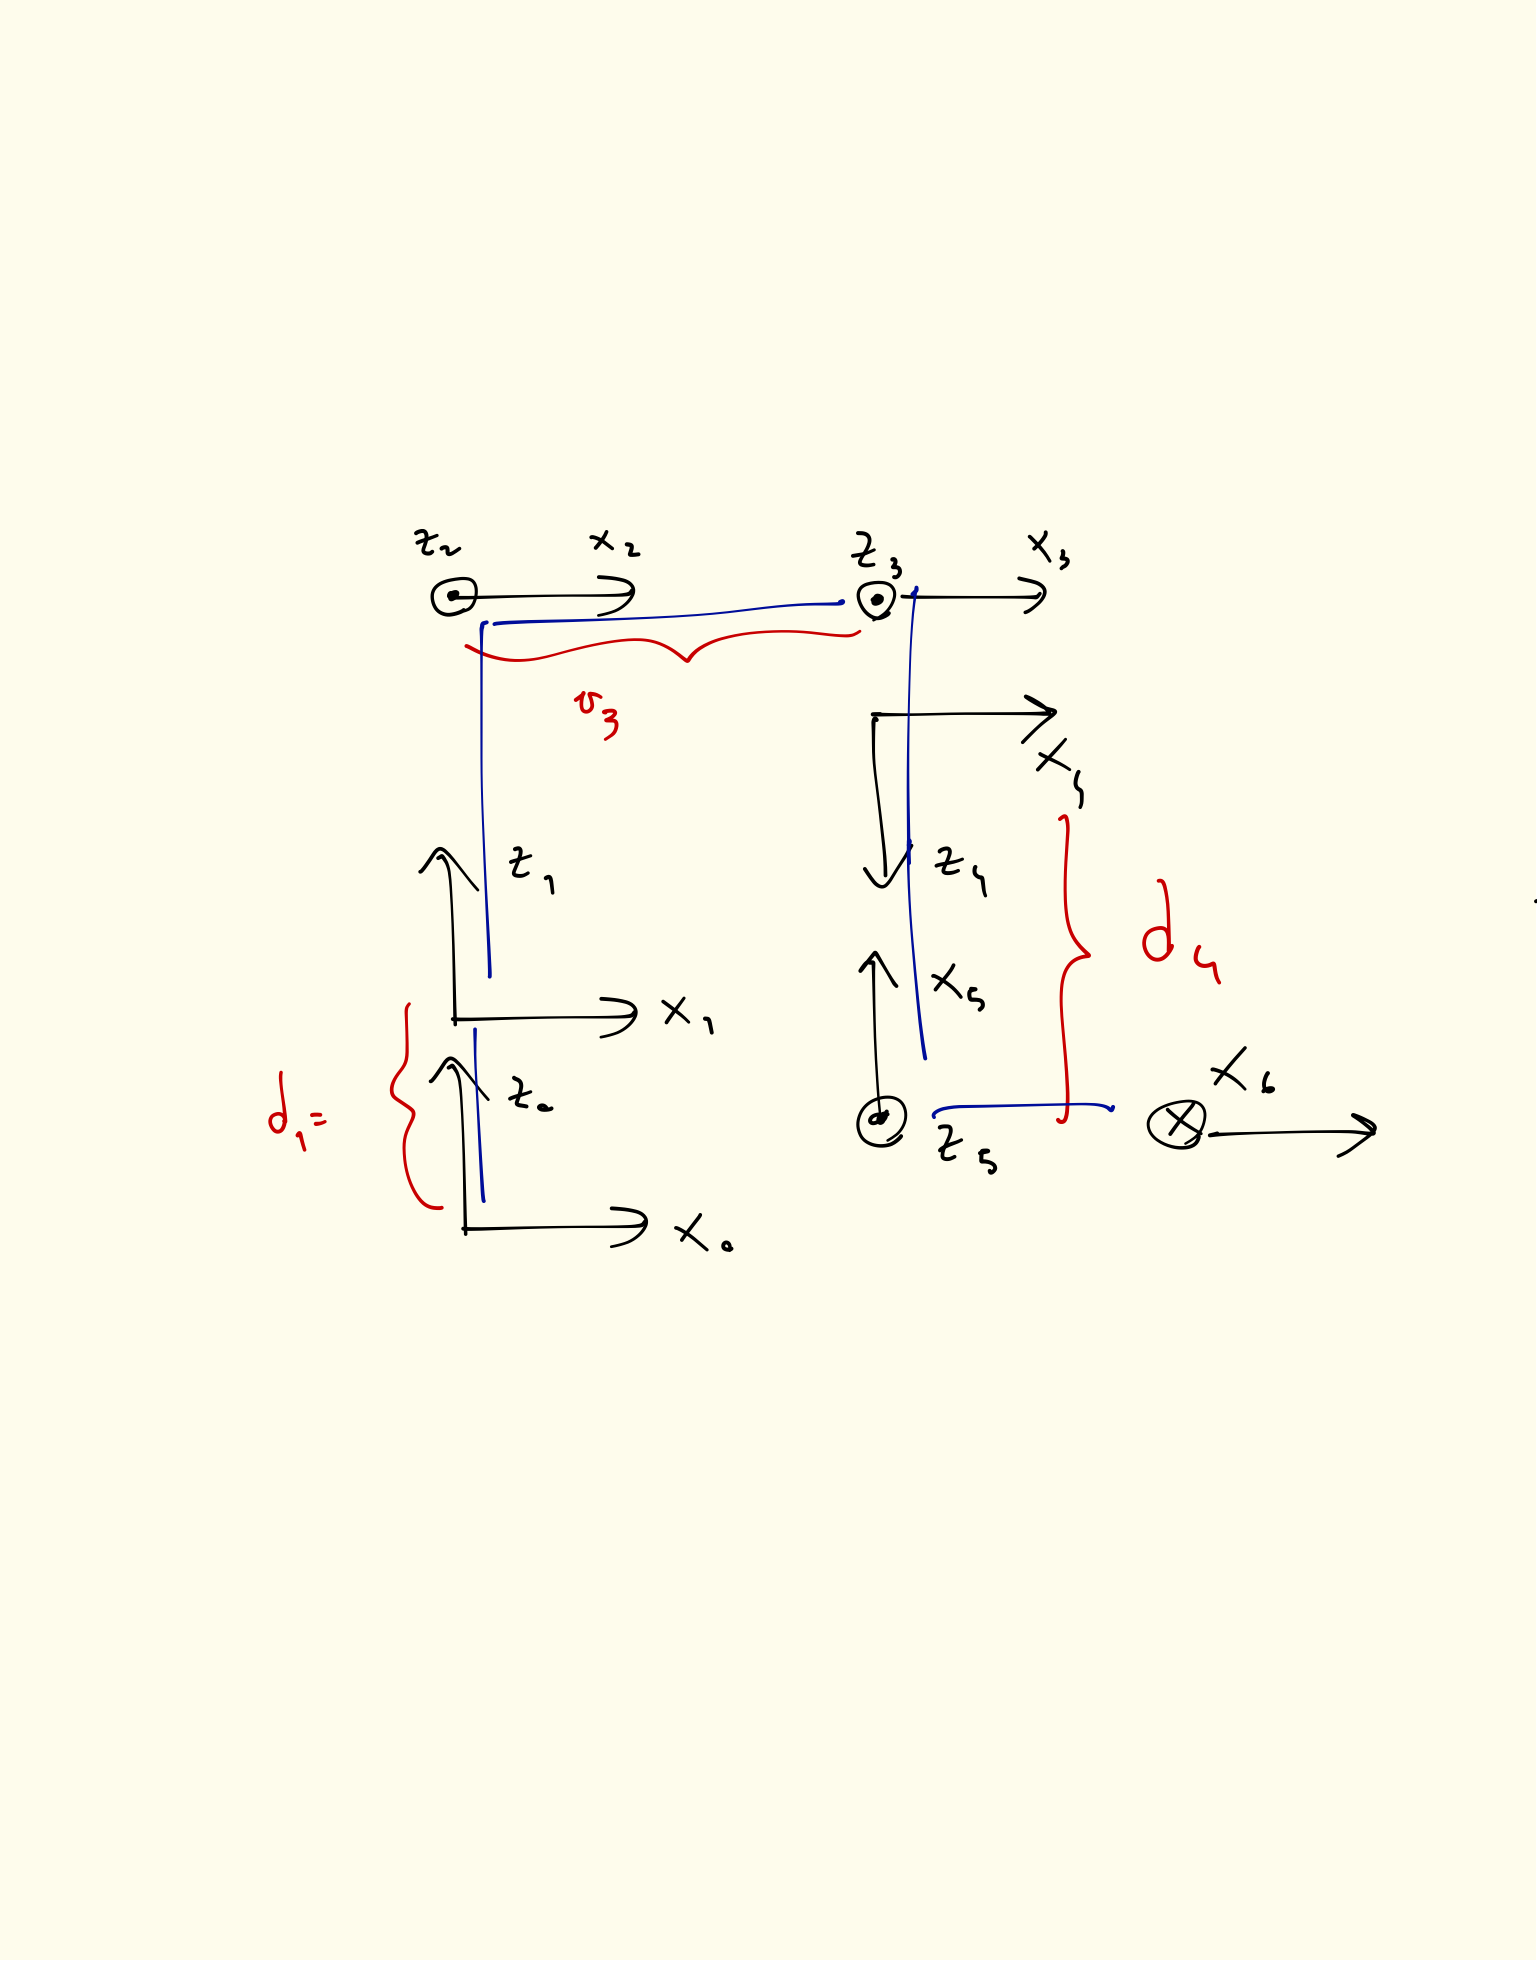
\includegraphics[width=\textwidth]{Geomagic_dh.png}
% 
\begin{scaletikzpicturetowidth}{0.85\textwidth}
\begin{tikzpicture}[scale=\tikzscale]

\node at (-0.25,-0.25) {$O_0$};
\draw [<->,ultra thick] (2,0) -- (0,0) -- (0,2);
\node at (2.5,0) {$x_0$};
\node at (-0.5,2) {$z_0$};

\draw [blue,thick, decorate,decoration={brace,amplitude=10pt},xshift=-4pt,yshift=0pt]
(-0.55,0) -- (-0.55,2.5) node [black,midway,xshift=-0.6cm] 
{\footnotesize $d_1$};

\draw [<->,ultra thick] (2,2.5) -- (0,2.5) -- (0,4.5);
\node at (2.5,2.5) {$x_1$};
\node at (-0.5,4.5) {$z_1$};

\draw [->,ultra thick] (0,6) -- (2,6);
\draw [fill=red] (0,6) circle [radius=0.1];
\draw [thick] (0,6) circle [radius=0.2];
\node at (0,6.6) {$z_2$};
\node at (2,6.6) {$x_2$};

\draw [blue,thick,decorate,decoration={brace,amplitude=10pt,mirror,raise=4pt},yshift=0pt]
(0,5.8) -- (5,5.8) node [black,midway,xshift=0cm,yshift=-0.7cm] {\footnotesize
$a_3$};

\draw [->,ultra thick] (5,6) -- (7,6);
\draw [fill=red] (5,6) circle [radius=0.1];
\draw [thick] (5,6) circle [radius=0.2];
\node at (5,6.6) {$z_3$};
\node at (7,6.6) {$x_3$};

\draw [<->,ultra thick] (5,2.5) -- (5,4.5) -- (7,4.5);
\node at (7,5) {$x_4$};
\node at (4.5,2.5) {$z_4$};

\draw [->,ultra thick] (5,0) -- (5,2);
\draw [fill=red] (5,0) circle [radius=0.1];
\draw [thick] (5,0) circle [radius=0.2];
\node at (4.5,0) {$z_5$};
\node at (4.5,2) {$x_5$};

\draw [blue,thick, decorate,decoration={brace,amplitude=10pt},xshift=-4pt,yshift=0pt]
(4.3,0) -- (4.3,4.5) node [black,midway,xshift=-0.6cm] 
{\footnotesize $d_4$};

\draw [->,ultra thick] (6.6,0) -- (8.5,0);
\draw [thick] (6.5,0) circle [radius=0.2];
\node [red, ultra thick] at (6.5,0) {x};
\node at (6.5,0.5) {$x_6$};

\draw [fill=red] (-1,-1) circle [radius=0.1];
\draw [thick] (-1,-1) circle [radius=0.2];
\node at (2.6,-0.95) {z axis outwards direction.};

\draw [thick] (-1,-1.5) circle [radius=0.2];
\node [red, ultra thick] at (-1,-1.5) {x};
\node at (2.5,-1.5) {z axis inwards direction.};

\end{tikzpicture}
\end{scaletikzpicturetowidth}

% \caption{Coordinate frame for the\newline Geomagic Touch.}
% \label{fig:Frame_phantom}
% \end{figure}
% \end{minipage}%\hfill
% \begin{minipage}[H]{.35\textwidth}




% \end{minipage}


\begin{figure}[H]

	\begin{subfigure}{.49\textwidth}
		\centering
		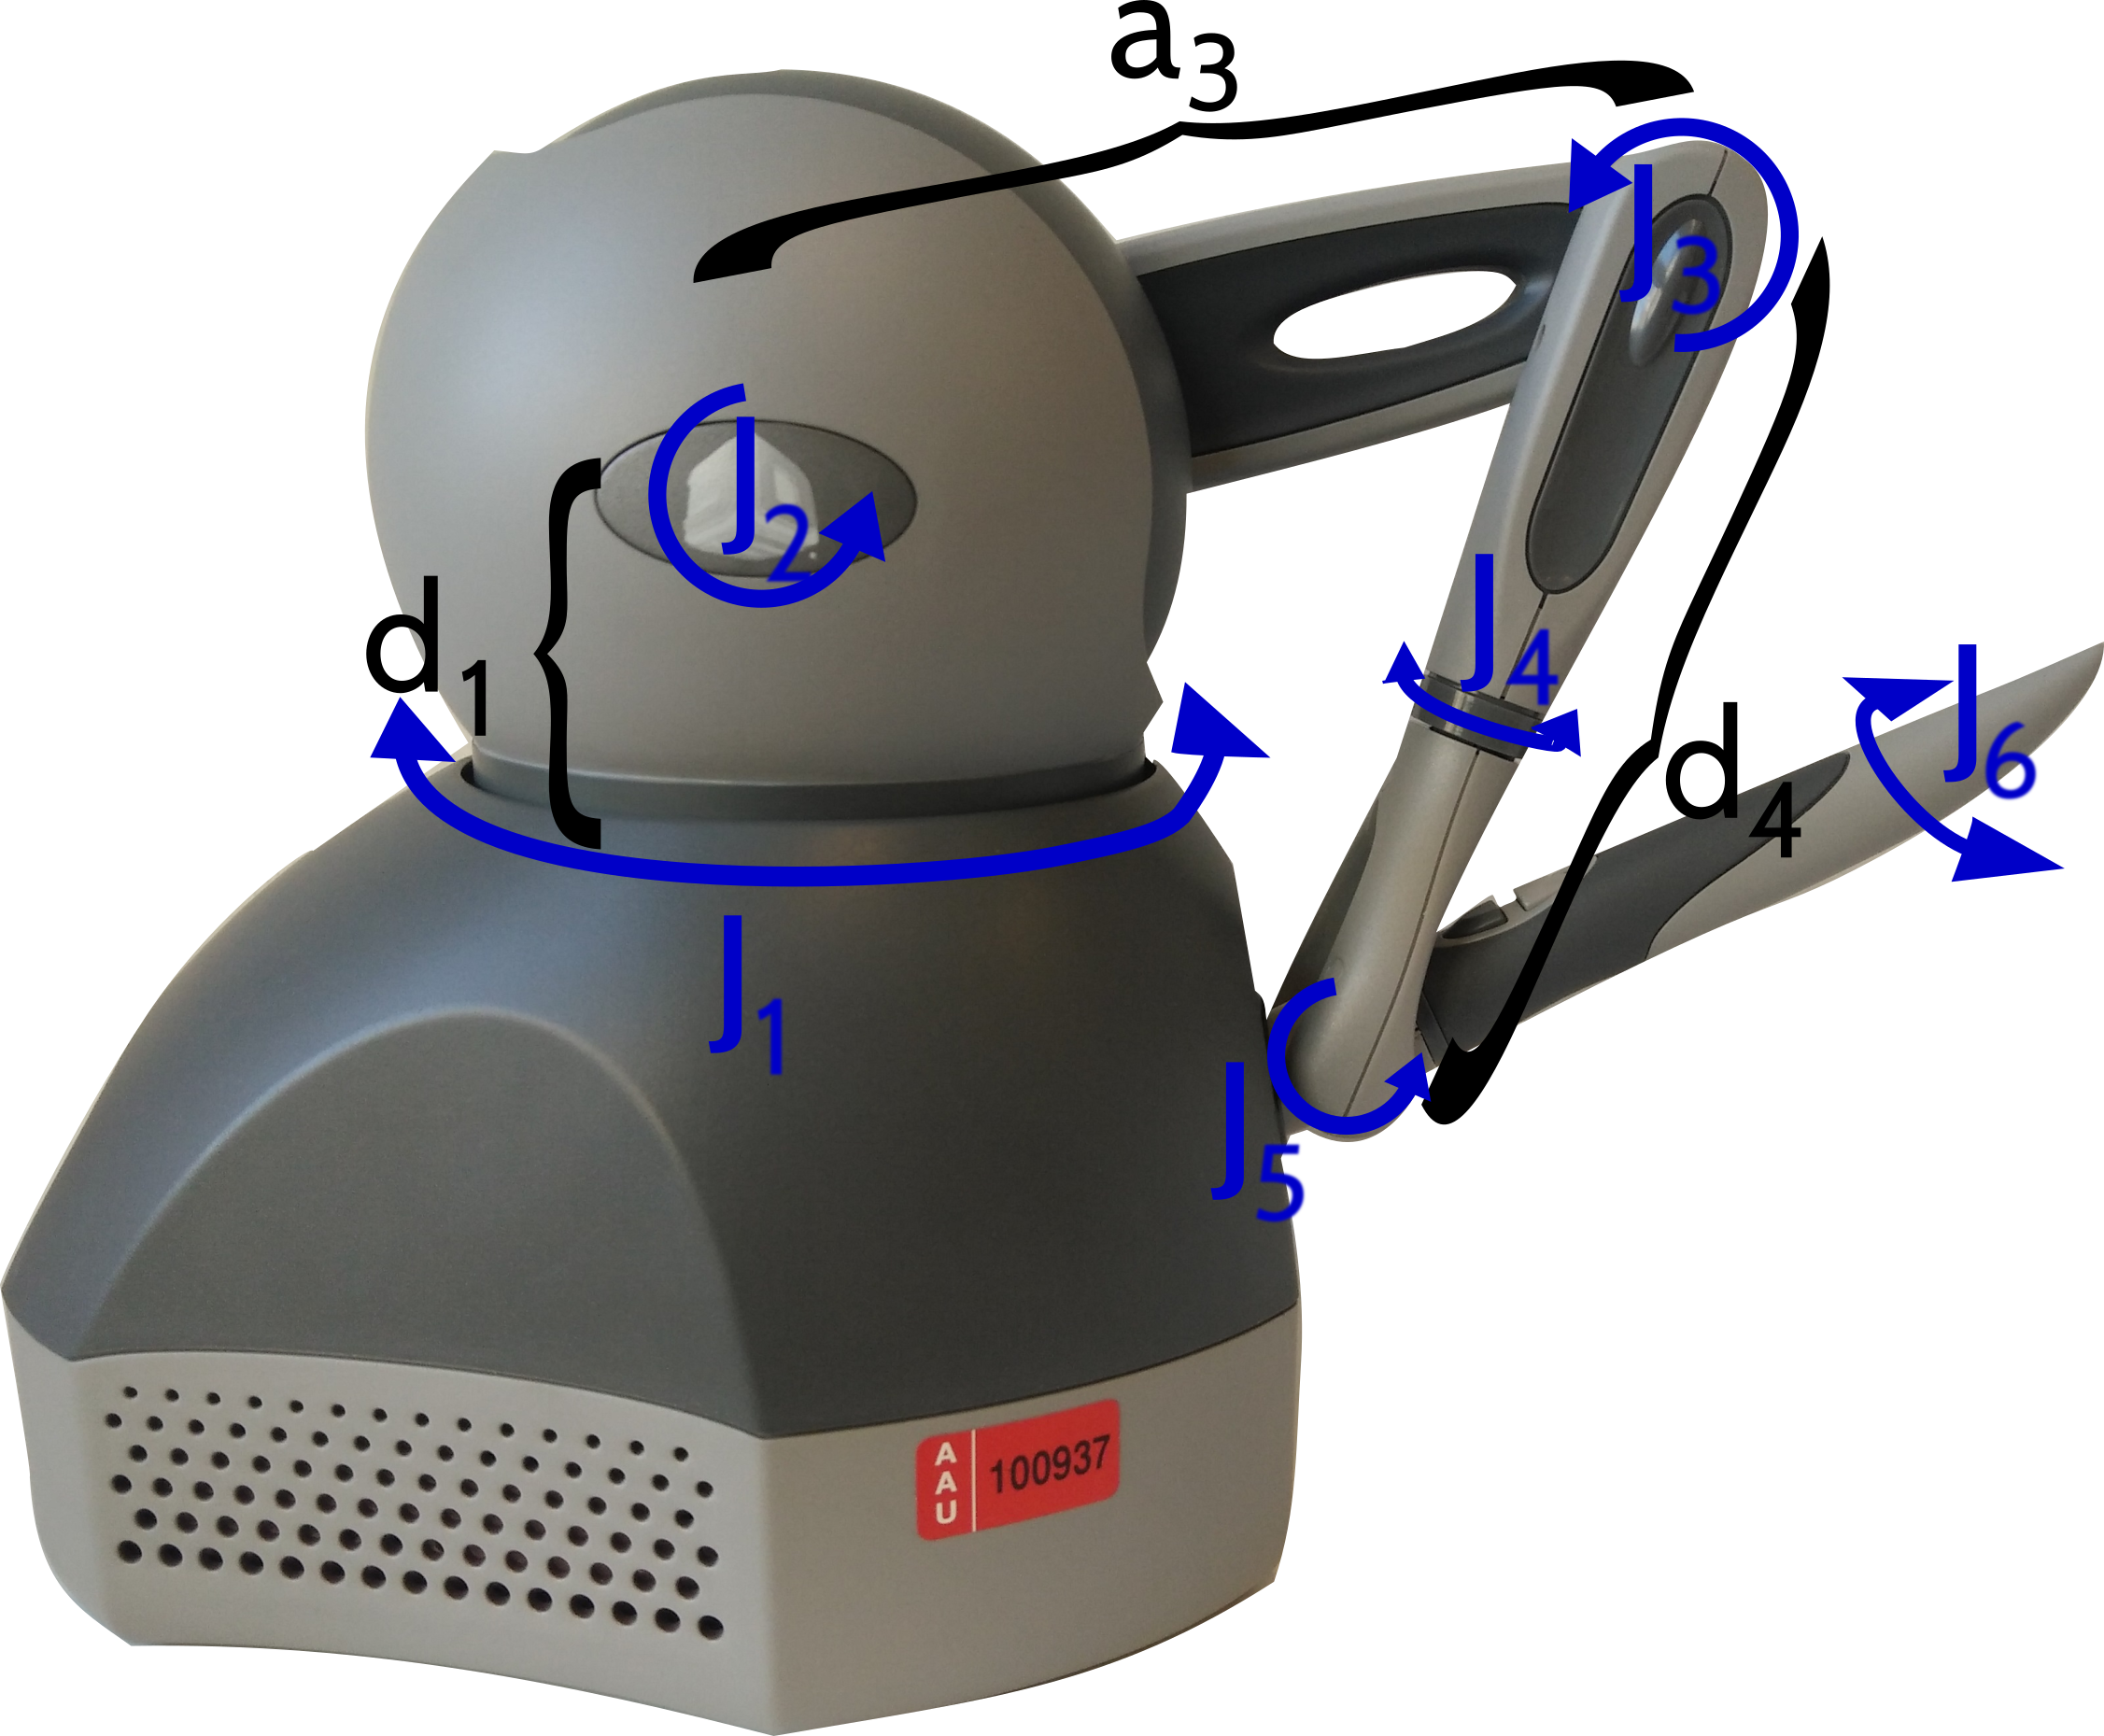
\includegraphics[width=\linewidth]{geo_kino.png}
		\caption{The Geomagic touch with defined joints numbers and the translations parameters.}
		\label{fig:Endo_plates11}
	\end{subfigure}
	\begin{subfigure}{.49\textwidth}
		\centering
		\vspace{5pt}
		
\begin{scaletikzpicturetowidth}{0.85\textwidth}
\begin{tikzpicture}[scale=\tikzscale]

\node at (-0.25,-0.25) {$O_0$};
\draw [<->,ultra thick] (2,0) -- (0,0) -- (0,2);
\node at (2.5,0) {$x_0$};
\node at (-0.5,2) {$z_0$};

\draw [blue,thick, decorate,decoration={brace,amplitude=10pt},xshift=-4pt,yshift=0pt]
(-0.55,0) -- (-0.55,2.5) node [black,midway,xshift=-0.6cm] 
{\footnotesize $d_1$};

\draw [<->,ultra thick] (2,2.5) -- (0,2.5) -- (0,4.5);
\node at (2.5,2.5) {$x_1$};
\node at (-0.5,4.5) {$z_1$};

\draw [->,ultra thick] (0,6) -- (2,6);
\draw [fill=red] (0,6) circle [radius=0.1];
\draw [thick] (0,6) circle [radius=0.2];
\node at (0,6.6) {$z_2$};
\node at (2,6.6) {$x_2$};

\draw [blue,thick,decorate,decoration={brace,amplitude=10pt,mirror,raise=4pt},yshift=0pt]
(0,5.8) -- (5,5.8) node [black,midway,xshift=0cm,yshift=-0.7cm] {\footnotesize
$a_3$};

\draw [->,ultra thick] (5,6) -- (7,6);
\draw [fill=red] (5,6) circle [radius=0.1];
\draw [thick] (5,6) circle [radius=0.2];
\node at (5,6.6) {$z_3$};
\node at (7,6.6) {$x_3$};

\draw [<->,ultra thick] (5,2.5) -- (5,4.5) -- (7,4.5);
\node at (7,5) {$x_4$};
\node at (4.5,2.5) {$z_4$};

\draw [->,ultra thick] (5,0) -- (5,2);
\draw [fill=red] (5,0) circle [radius=0.1];
\draw [thick] (5,0) circle [radius=0.2];
\node at (4.5,0) {$z_5$};
\node at (4.5,2) {$x_5$};

\draw [blue,thick, decorate,decoration={brace,amplitude=10pt},xshift=-4pt,yshift=0pt]
(4.3,0) -- (4.3,4.5) node [black,midway,xshift=-0.6cm] 
{\footnotesize $d_4$};

\draw [->,ultra thick] (6.6,0) -- (8.5,0);
\draw [thick] (6.5,0) circle [radius=0.2];
\node [red, ultra thick] at (6.5,0) {x};
\node at (6.5,0.5) {$x_6$};

\draw [fill=red] (-1,-1) circle [radius=0.1];
\draw [thick] (-1,-1) circle [radius=0.2];
\node at (2.6,-0.95) {z axis outwards direction.};

\draw [thick] (-1,-1.5) circle [radius=0.2];
\node [red, ultra thick] at (-1,-1.5) {x};
\node at (2.5,-1.5) {z axis inwards direction.};

\end{tikzpicture}
\end{scaletikzpicturetowidth}

		\caption{The different frames for the Geomagic touch.}
		\label{fig:dhgeoframe1}
	\end{subfigure}
\caption{Shows joints positions, the translations \gls{DH} parameters and the coordinate frame for each joint. The base frame is difined as $O_{0}$.}
\label{fig:dhnotatso2}
\end{figure}



The DH notations for the Geomagic touch, can be derived as shown in \tabref{tab:kin_geo}.





\begin{table}[H]
\centering
\begin{tabular}{|l|l|l|l|l|}
\hline
 $j_i$ 	  & $a_i$    & $d_i$ & $\alpha_i$ 		 & $\theta_i$ 			 	\\ \hline
 1  	  &  $0$     & $d_1$ & $0$	 			 & $q_1$ 			    	 \\ \hline
 2  	  &  $0$     & $0$ 	 & $\frac{\pi}{2}$ 	 & $q_2 + \theta_1$ 		 \\ \hline
 3  	  &  $a_3$	 & $0$   & $0$ 		 		 & $q_3$ 					  \\ \hline
 4  	  &  $0$	 & $d_4$ & $\frac{\pi}{2}$ 	 & $q_4$ 			 		  \\ \hline
 5  	  &  $0$	 & $0$   & $-\frac{\pi}{2}$  & $-\frac{\pi}{2} + q_5$	 \\ \hline
 6  	  &  $0$	 & $0$   & $-\frac{\pi}{2}$  & $\frac{\pi}{2}+q_6$ 		 \\ \hline
\end{tabular}
\hspace{2cm}\caption{The DH notations for the\newline Geomagic Touch}
\label{tab:kin_geo}
\end{table}




% \begin{figure}[H]
% 	\centering
% 	\begin{subfigure}{.49\textwidth}
% 		\centering
% 		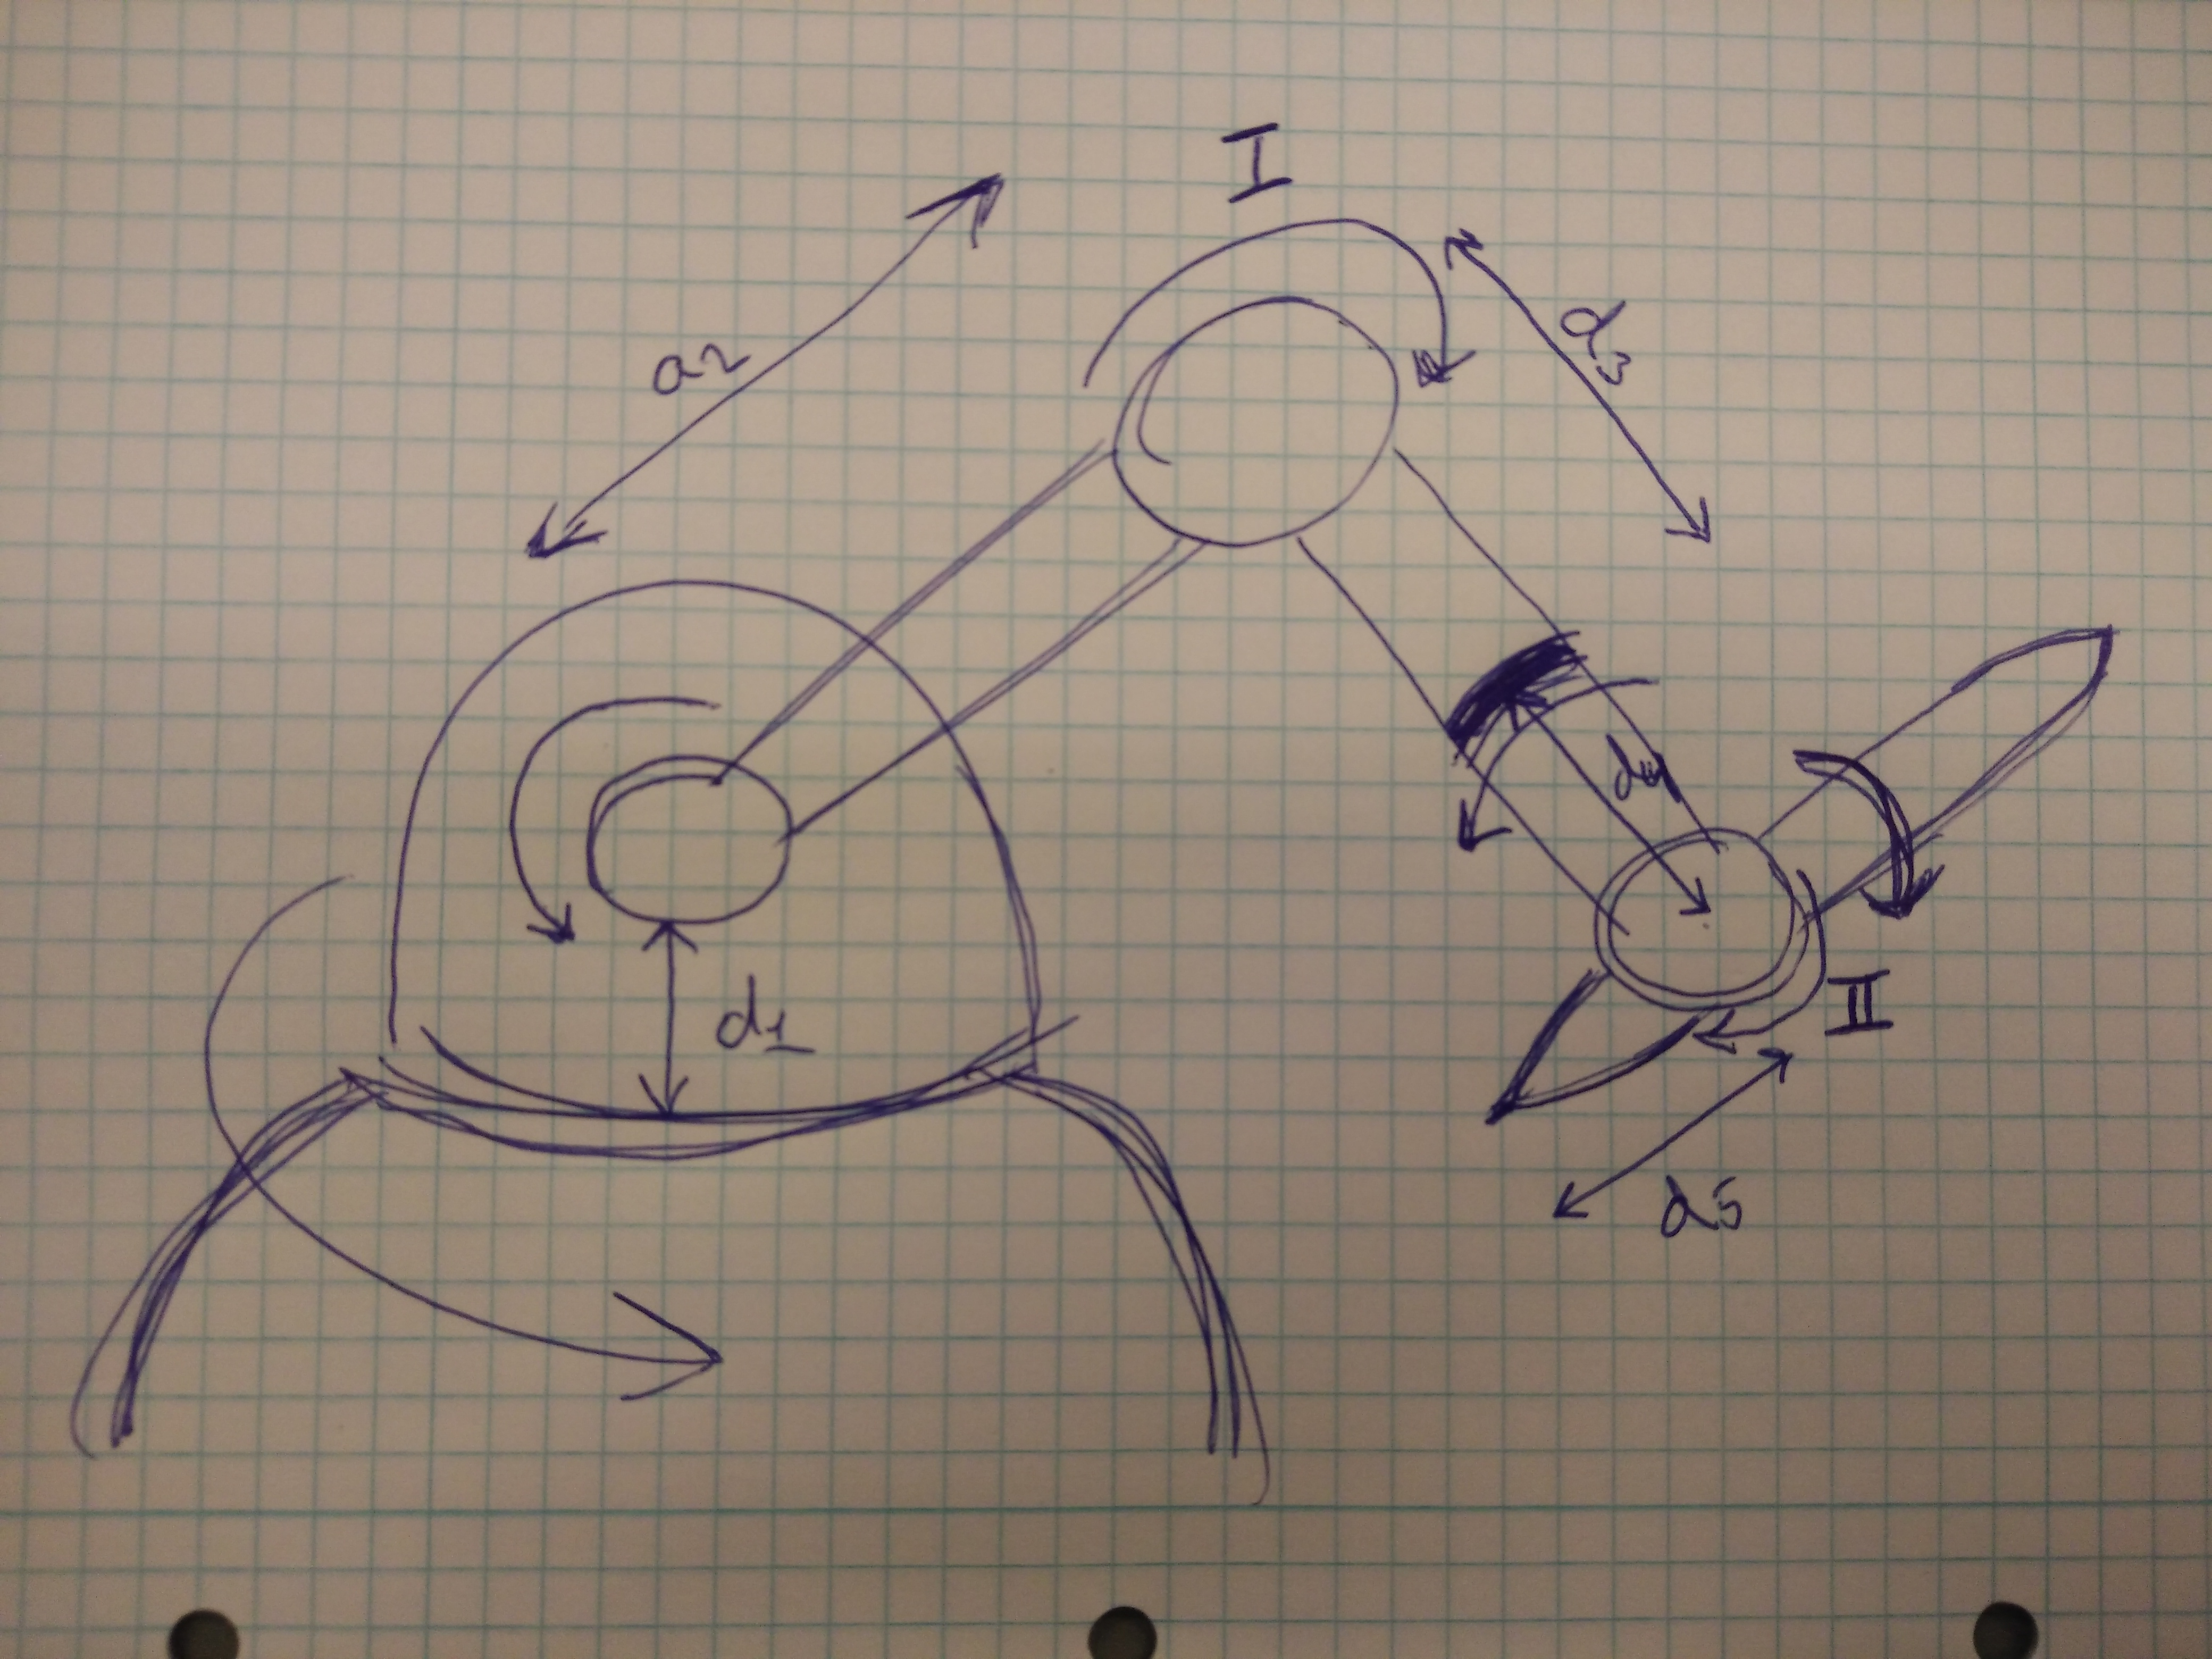
\includegraphics[width=\linewidth]{Fast_draw_Kino.jpg}
% 		\caption{Geomagic touch with all rotational joints and their \gls{DH} parameters.}
% 		\label{fig:1}
% 	\end{subfigure}
% 	\begin{subfigure}{.49\textwidth}
% 		\centering
% 		\includegraphics[width=\linewidth]{Fast_draw_kino2.jpg}
% 		\caption{Frame coordinate system for the Geomagic touch to the deviation of the kinematics.}
% 		\label{fig:Endo_plates}
% 	\end{subfigure}
% \caption{Shows joints positions, the different \gls{DH} parameters and the coordinate frame for each joint. The base frame is difined as $O_{0}$.}
% \label{fig:2}
% \end{figure}


% \begin{table}[H]
% \centering
% \begin{tabular}{|l|l|l|l|l|}
% \hline
%  $j_i$ 	  & $a_i$    & $d_i$ & $\alpha_i$ 		 & $\theta_i$ 			 \\ \hline
%  1  	  &  $0$     & $d_1$ & $\frac{\pi}{2}$	 & $q_1$ 			     \\ \hline
%  2  	  &  $a_2$   & $0$ 	 & $0$ 		 		 & $q_2 + \theta_1$ 	 \\ \hline
%  \rom{1}  &  $0$	 & $0$ 	 & $\frac{\pi}{2}$ 	 & $\frac{\pi}{2} + q_3$ \\ \hline
%  3  	  &  $0$	 & $d_3$ & $0$ 		 		 & $0$ 					 \\ \hline
%  4  	  &  $0$	 & $d_4$ & $\frac{\pi}{2}$ 	 & $\pi + q_4$ 			 \\ \hline
%  \rom{2}  &  $0$	 & $0$ 	 & $\frac{\pi}{2}$   & $\pi +q_5$ 			 \\ \hline
%  5  	  &  $0$	 & $d_5$ & $0$ 		 		 & $0$ 	 				 \\ \hline
%  %6  	  &  $0$	 & $d_6$ & $\theta$ 		 & $q_6$ 				 \\ \hline
% \end{tabular}
% \caption{Tabular which contain the kinematics for the Geomagic touch described in \secref{sec:geo_magic}.The Roman numbers defines the fictional joints}
% \label{tab:kin_geo}
% \end{table}

%%%\section{Kinematics for the Endowrist}


\section{Kinematics for the Da vinci robot}
This section is covering the derivation of one hand of the da Vinci robot.

It can be seen on \figref{fig:da_hand_kino}, at the end of the hand there is marked a stationary point. This point is seen as the reference point for the hand. The hand has three DOF where two of them is rotations and the last one is the translation. Both rotations can be put at the stationary point due to the fact that each rotation will not translate the stationary point of the hand. The translation is handling the position of the end-effector in respect to the reference point, where the distance is marked as $d_3$ on \figref{fig:da_hand_kino}.

The DH parameters for the da Vinci hand can be seen on \tabref{tab:DH_notation_hand} as two rotations and one translation.

\begin{figure}[H]
		\centering
		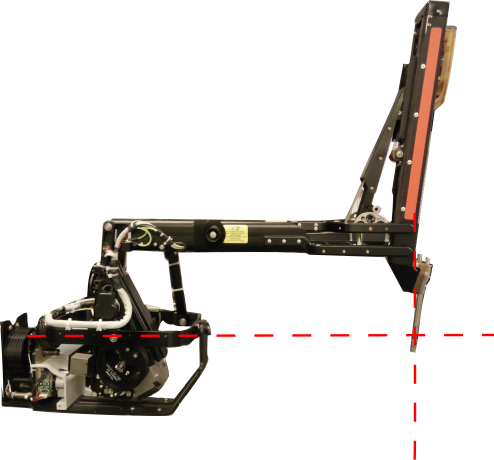
\includegraphics[width=0.6\linewidth]{Hand_davinci_robot.png}
		\caption{The da Vinci hand. The cross section shows the stationary reference for the hand. The blue arrows illustrate the two rotations in in the reference point. The green arrow is the movement of the Endo-Wrist and $d_3$ is the distance between the reference and end-effector.}
		\label{fig:da_hand_kino}
\end{figure}


\begin{table}[H]
\centering
\begin{tabular}{|l|l|l|l|l|}
	\hline
 	$j_i$ 	  & $a_i$    & $d_i$ & $\alpha_i$ 		 & $\theta_i$ 			   	 \\ \hline
 	1  	  	  &  $0$     & $0$ 	 & $-\frac{\pi}{2}$	 		 & $q_1$ 			    	 \\ \hline
 	2  		  &  $0$   	 & $0$ 	 & $ \frac{\pi}{2}$ 	 & $\frac{\pi}{2}+q_2$ 		 \\ \hline
 	3 	 	  &  $0$	 & $d_3$ & $0$ 		 		 & $0$ 					 \\ \hline
\end{tabular}
\caption{The DH notations for the da Vinci hand.}
\label{tab:DH_notation_hand}
\end{table}


